% calculus:x12 GDC:NO
\begin{question}
  \hspace*{\fill} [Note maximale: 17]\par
  \medskip
  \noindent Soit $f(x) = 6 + 6$ sin $x$. Une partie de la representation grafique the $f$ est donnée ci-dessous.\par
  \medskip
  \begin{center}
    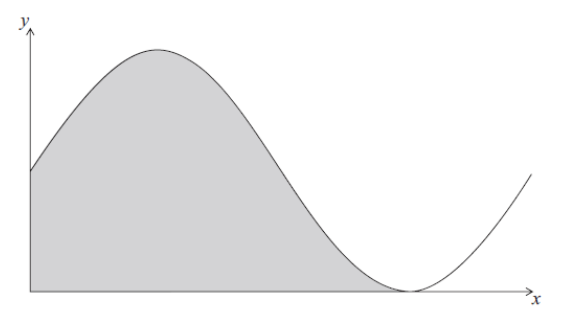
\includegraphics[scale=0.3]{temp_6_plus_6sinx}\par
  \end{center}
  \medskip
  \noindent La région grisée est limitée par la courbe représentant $f$, l’axe des abscisses et l’axe des ordonnées.\par
  \medskip
  (a) Resolvez, avec $0 \le x \le 2\pi$\par
  \hspace{1em} (i ) $6$ + sin $x = 6$;\par
  \hspace{1em} (ii) $6$ + sin $x = 0$.\hspace*{\fill} [5]\par
  \medskip
  (b) Donnez la valeur exacte de l’abscisse à l’origine de $f$, avec $0 \le x \le 2\pi$.\hspace*{\fill} [1]\par
  \medskip
  (c) L’aire de la région grisée est $k$. Trouvez la valeur de $k$, en donnant votre réponse en fonction de $\pi$.\hspace*{\fill} [6]\par
  \medskip
  \noindent Soit $g(x) = 6 + 6$ sin $(x - \frac{\pi}{2})$. La representation graphique the $f$ est transformeé en celle de $g$.\par
  \medskip
  (d) Donnez une description géométrique complète de cette transformation.\hspace*{\fill} [2]\par
  \medskip
  (e) Étant donné que $\int_p^{p+\frac{3\pi}{2}}g(x)\,dx =k$ et $0 \le p < 2\pi$, donnez les deux valeur de $p$.\hspace*{\fill} [3]\par
\end{question}


